\documentclass[12pt,a4paper]{ctexart}

\usepackage[a4paper,top=2.5cm,bottom=2.5cm,left=2.4cm,right=2.4cm]{geometry}
\usepackage{xcolor}
\usepackage{graphicx}
\usepackage{booktabs}
\usepackage{array}
\usepackage{float}
\usepackage{amsmath}
\usepackage{hyperref}
\usepackage{fancyhdr}
\usepackage{titlesec}
\usepackage{enumitem}
\usepackage{caption}
\usepackage{subcaption}
\usepackage{listings}
\usepackage{tikz}
\usetikzlibrary{arrows.meta,positioning,shapes.geometric,calc}

\hypersetup{
  colorlinks=true,
  linkcolor=blue!50!black,
  urlcolor=blue!50!black,
  pdftitle={实验七 温度采集控制器实验报告},
  pdfauthor={自动化学院}
}

\definecolor{themecolor}{RGB}{18,77,125}
\definecolor{accentred}{RGB}{178,34,34}
\definecolor{accentgreen}{RGB}{28,128,70}
\definecolor{accentyellow}{RGB}{180,128,0}
\definecolor{softline}{RGB}{220,228,236}
\definecolor{codebg}{RGB}{246,248,250}
\definecolor{codekw}{RGB}{0,92,175}
\definecolor{codecmt}{RGB}{24,120,58}

\titleformat{\section}{\Large\bfseries\color{themecolor}}{\thesection}{0.8em}{}
\titleformat{\subsection}{\large\bfseries\color{themecolor}}{\thesubsection}{0.6em}{}
\titlespacing*{\section}{0pt}{1.2em}{0.7em}
\titlespacing*{\subsection}{0pt}{0.9em}{0.5em}

\captionsetup{font={small,bf},labelsep=quad}
\setlist[enumerate]{itemsep=0.35em,topsep=0.35em,leftmargin=2em}
\setlist[itemize]{itemsep=0.3em,topsep=0.3em,leftmargin=2em}

\pagestyle{fancy}
\fancyhf{}
\fancyhead[L]{\small 实验七\quad 温度采集控制器实验}
\fancyhead[R]{\small 微机原理与接口技术}
\fancyfoot[C]{\thepage}
\setlength{\headheight}{25pt}
\renewcommand{\headrulewidth}{0.5pt}
\renewcommand{\headrule}{\hbox to\headwidth{\color{softline}\leaders\hrule height \headrulewidth\hfill}}

\lstdefinelanguage{A51}{
  morekeywords={ORG,LJMP,JMP,SJMP,START,MAIN,LOOP,MOV,SETB,CLR,LCALL,CALL,DJNZ,PUSH,POP,RET,RETI,END,DELAY,DB,CJNE,JNC,JC,JNB,JB,NOP,DIV,MUL,SUBB,ADD,MOVC,EQU,P0,P1,P2,P3,SP,DPTR,ACC,B,R6,R7,A},
  sensitive=false,
  morecomment=[l]{;}
}

\lstdefinestyle{a51style}{
  language=A51,
  basicstyle=\ttfamily\small,
  keywordstyle=\color{codekw}\bfseries,
  commentstyle=\color{codecmt}\itshape,
  numbers=left,
  numberstyle=\tiny\color{gray},
  stepnumber=1,
  numbersep=8pt,
  backgroundcolor=\color{codebg},
  frame=single,
  framerule=0.4pt,
  rulecolor=\color{softline},
  showstringspaces=false,
  breaklines=true,
  tabsize=4
}

\newcommand{\CourseName}{微机原理与接口技术}
\newcommand{\CollegeName}{自动化学院}
\newcommand{\MajorName}{自动化（新工科试验班）}
\newcommand{\StudentID}{24061428}
\newcommand{\StudentName}{张跃哲}
\newcommand{\TeacherName}{金朝阳}
\newcommand{\FinishDate}{2026年6月21日}

\begin{document}

\begin{titlepage}
  \thispagestyle{empty}
  \begin{tikzpicture}[remember picture,overlay]
    \node[anchor=north east,inner sep=0pt] at ([xshift=-1.4cm,yshift=-1.2cm]current page.north east) {
\includegraphics[width=2.5cm]{images/hdu_motto.jpg}};
  \end{tikzpicture}

  \centering
  \vspace*{0.8cm}
  
\includegraphics[width=4.6cm]{images/hdu_logo.pdf}\par

  \vspace{1.1cm}
  {\zihao{4}\bfseries 杭州电子科技大学\par}

  \vspace{1.1cm}
  {\zihao{-1}\bfseries 实验七\quad 温度采集控制器实验报告\par}

  \vspace{2.4cm}
  \renewcommand{\arraystretch}{1.8}
  \begin{tabular}{>{\raggedleft\arraybackslash}p{3.2cm}p{8.2cm}}
    课程 & \CourseName \\
    学院 & \CollegeName \\
    专业 & \MajorName \\
    学号 & \StudentID \\
    学生姓名 & \StudentName \\
    指导教师 & \TeacherName \\
    完成日期 & \FinishDate \\
  \end{tabular}

  \vfill
\end{titlepage}

\pagenumbering{Roman}
\tableofcontents
\clearpage

\pagenumbering{arabic}
\setcounter{page}{1}

\section{实验要求与实验目的}

\subsection{实验要求}
本实验要求利用 AT89C51 单片机、ADC0808 模数转换器和 AT502 热敏电阻构成温度采集控制器。系统通过热敏电阻分压电路把温度变化转换为模拟电压，再由 ADC0808 转换为 8 位数字量，最后由单片机处理后送至最左侧两位共阴极八段数码管显示。根据实验说明和开发板资源限制，本实验采用如下连接关系：
\begin{enumerate}
  \item ADC0808 的 8 位数据输出口接 AT89C51 的 P1.0--P1.7。
  \item ADC0808 的 OE 接 P2.1，START 与 ALE 共接 P2.2，EOC 接 P3.4。
  \item ADC0808 的 CLOCK 引脚由 Proteus 数字时钟源提供 500kHz 方波。
  \item 温度传感器采用 5k$\Omega$ NTC 热敏电阻，经过分压后接 ADC0808 的 IN0 通道。
  \item 显示部分使用最左边两只共阴极数码管显示温度值。
\end{enumerate}

\subsection{实验目的}
\begin{enumerate}
  \item 理解 A/D 转换的基本过程，掌握模拟量采样、量化和数字量读取之间的关系。
  \item 熟悉 ADC0808 的通道选择、启动转换、结束判断和输出允许控制方法。
  \item 掌握 AT89C51 定时器中断、并行 I/O 口和动态数码管显示的综合应用。
  \item 理解热敏电阻分压测温的基本原理，并能够在 Proteus 中完成电路与程序联合调试。
\end{enumerate}

\subsection{总体方案}
系统以 AT89C51 为控制核心。热敏电阻与固定电阻构成分压网络，温度改变时热敏电阻阻值变化，ADC0808 的 IN0 输入电压随之改变。单片机每隔 1s 通过 P2.2 向 ADC0808 发出 START/ALE 脉冲，等待 P3.4 接收到转换完成信号后，打开 P2.1 对应的 OE 控制端，从 P1 口读入 8 位转换结果。程序将 ADC 值近似换算为温度值，并通过 P0 总线和两片 74HC573 锁存器驱动数码管动态显示。

\begin{figure}[H]
\centering
\resizebox{\textwidth}{!}{%
\begin{tikzpicture}[
  node distance=10mm and 14mm,
  block/.style={rectangle,rounded corners,draw=themecolor,fill=blue!3,minimum width=3.6cm,minimum height=9mm,align=center},
  io/.style={trapezium,trapezium left angle=75,trapezium right angle=105,draw=accentgreen,fill=green!8,minimum width=3.8cm,minimum height=9mm,align=center},
  line/.style={-Latex,thick,draw=themecolor}
]
  \node[io] (temp) {AT502\\热敏电阻};
  \node[block,right=of temp] (divider) {电阻分压\\模拟电压};
  \node[block,right=of divider] (adc) {ADC0808\\A/D 转换};
  \node[block,right=of adc] (mcu) {AT89C51\\定时采集与换算};
  \node[io,right=of mcu] (seg) {最左两位\\数码管显示};

  \draw[line] (temp) -- (divider);
  \draw[line] (divider) -- node[above,font=\small] {IN0} (adc);
  \draw[line] (adc) -- node[above,font=\small] {P1 数据口} (mcu);
  \draw[line] (mcu) -- node[above,font=\small] {P0 + 74HC573} (seg);
\end{tikzpicture}}
\caption{温度采集控制器总体结构}
\end{figure}

\section{硬件电路设计}

\subsection{单片机最小系统}
AT89C51 采用 +5V 供电，XTAL1 与 XTAL2 外接晶振和两个 30pF 电容构成时钟电路。EA 端通过电阻接 +5V，使单片机从片内程序存储器取指。RST 引脚连接复位网络，保证上电或按键复位时程序能够从 0000H 地址重新执行。该部分是单片机稳定运行的基础。

\begin{figure}[H]
  \centering
  \begin{subfigure}{0.58\textwidth}
    \centering
    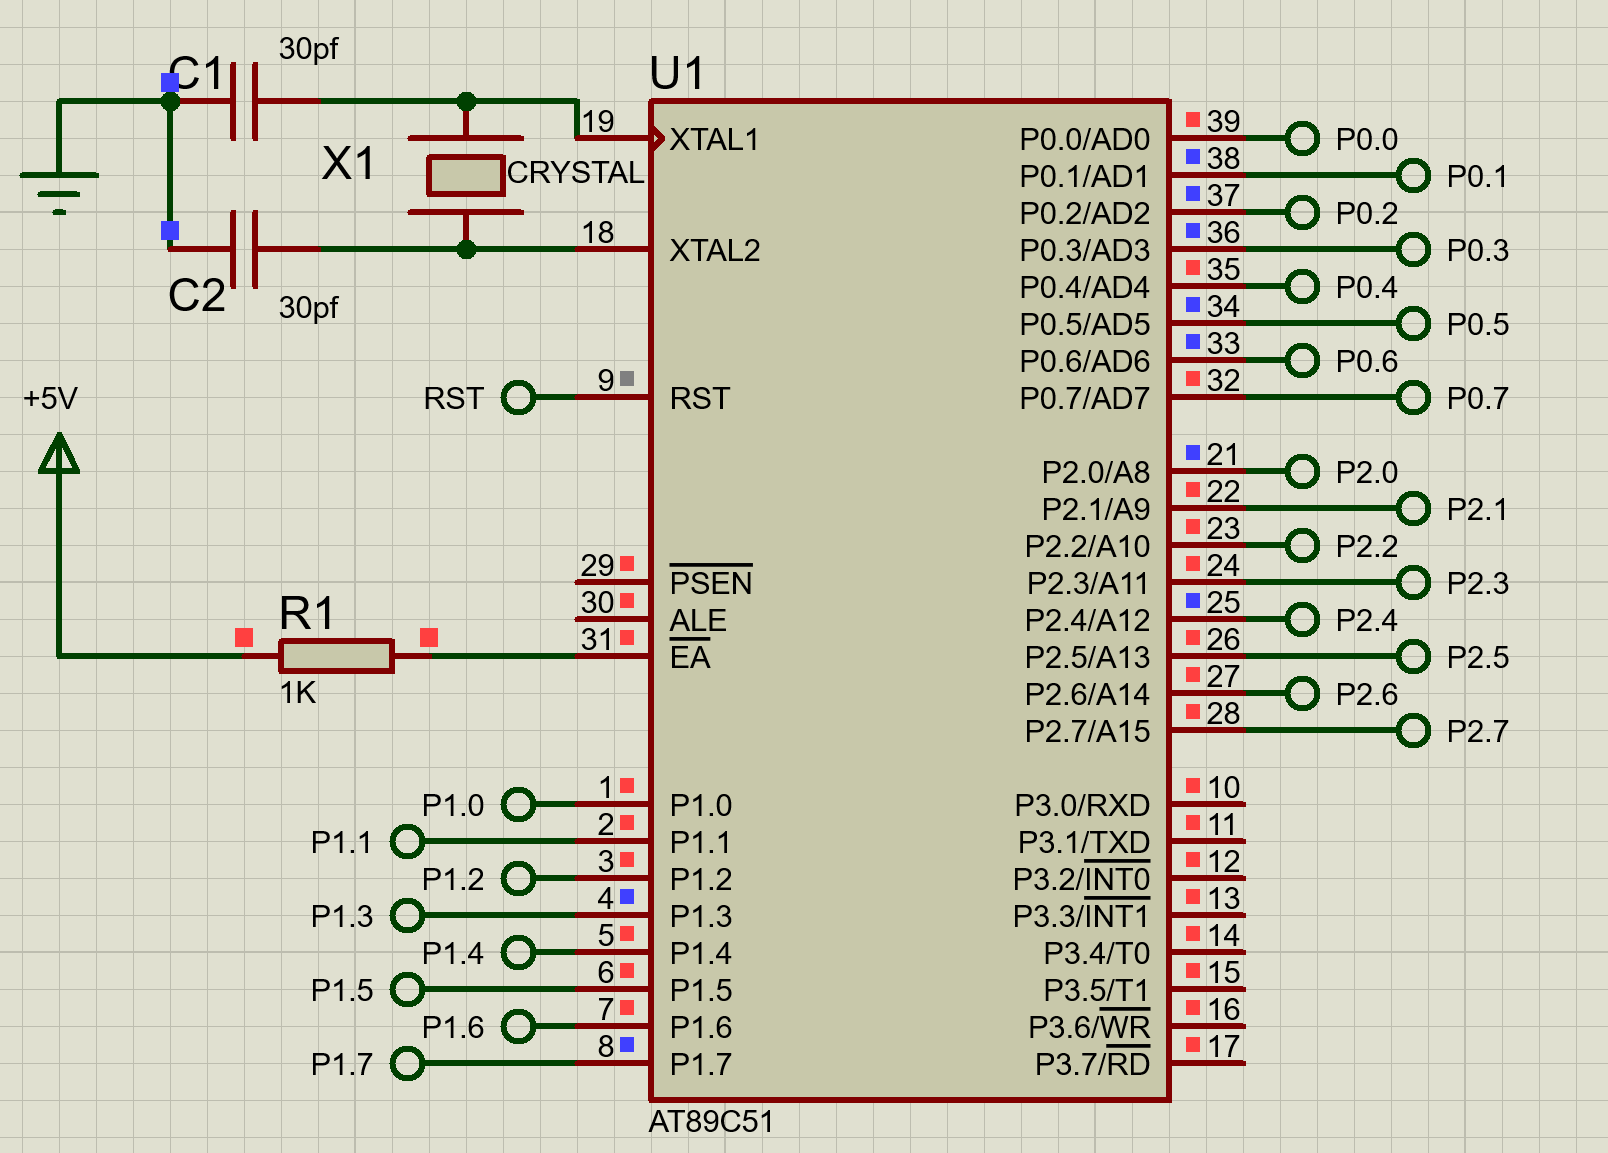
\includegraphics[width=\textwidth]{images/power.png}
    \caption{AT89C51 供电与晶振电路}
  \end{subfigure}
  \hfill
  \begin{subfigure}{0.34\textwidth}
    \centering
    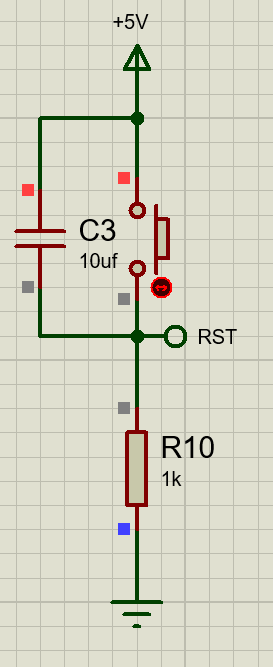
\includegraphics[width=\textwidth]{images/rst.png}
    \caption{复位电路}
  \end{subfigure}
  \caption{单片机最小系统基础电路}
\end{figure}

\subsection{温度采集与 ADC0808 接口}
ADC0808 采用 8 位逐次逼近式 A/D 转换结构，具有 IN0--IN7 八路模拟输入。由于本实验只采集一路温度信号，因此 ADD A、ADD B、ADD C 全部接地，固定选择 IN0 通道。VREF(+) 接 +5V，VREF(-) 接 GND，因此转换结果满足近似关系：
\[
  D = \frac{V_{\text{IN0}}}{5V} \times 255
\]
其中 $D$ 为 P1 口读到的 8 位 ADC 数值。

温度分压采用固定上拉电阻与 NTC 热敏电阻构成。若上拉电阻为 $R_3$，热敏电阻为 $R_T$，则 IN0 电压为：
\[
  V_{\text{IN0}} = 5V \times \frac{R_T}{R_3 + R_T}
\]
NTC 热敏电阻温度升高时阻值下降，因此 IN0 电压和 ADC 数值也随温度升高而下降。为了便于仿真调试，可用电位器代替热敏电阻进行阻值变化模拟，但不宜将电位器、固定电阻和热敏电阻随意串联，否则分压关系会偏离测温模型。

\begin{figure}[H]
  \centering
  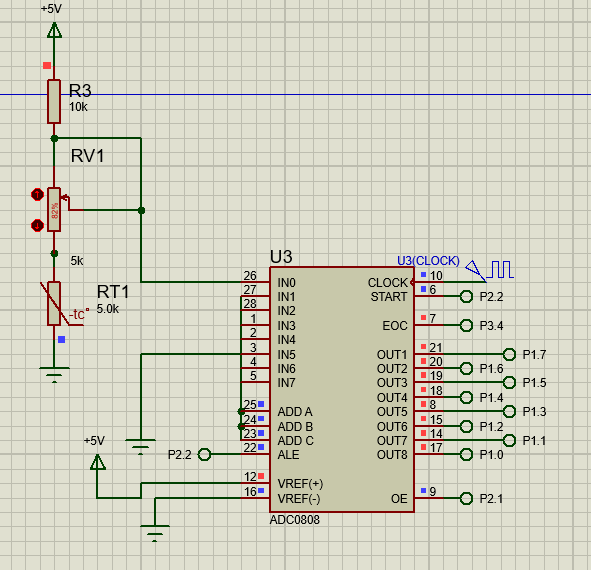
\includegraphics[width=0.78\textwidth]{images/ADC0805.png}
  \caption{ADC0808 温度采集接口电路}
\end{figure}

\subsection{ADC0808 控制时序}
本实验将 START 与 ALE 共接 P2.2。采样时，单片机先使 P2.2 产生一个高电平脉冲，ADC0808 锁存通道地址并开始转换；随后程序检测 EOC 引脚状态，等待转换完成；最后置位 OE，使 ADC0808 将转换结果输出到 P1 口。读取完成后关闭 OE，避免数据总线长期被外设驱动。

\begin{figure}[H]
\centering
\begin{tikzpicture}[
  node distance=8mm,
  stepnode/.style={rectangle,rounded corners,draw=themecolor,fill=blue!3,minimum width=8.4cm,minimum height=8mm,align=center},
  check/.style={diamond,aspect=2.3,draw=accentyellow,fill=yellow!10,minimum width=4.3cm,minimum height=10mm,align=center},
  line/.style={-Latex,thick,draw=themecolor}
]
  \node[stepnode] (s1) {P1 写 0FFH，释放数据口为输入状态};
  \node[stepnode,below=of s1] (s2) {P2.2 输出 START/ALE 高脉冲};
  \node[check,below=of s2] (s3) {EOC 是否完成转换};
  \node[stepnode,below=of s3] (s4) {P2.1 置 1，打开 OE};
  \node[stepnode,below=of s4] (s5) {从 P1 读取 8 位 ADC 数据};
  \node[stepnode,below=of s5] (s6) {P2.1 清 0，关闭 OE};

  \draw[line] (s1) -- (s2);
  \draw[line] (s2) -- (s3);
  \draw[line] (s3) -- node[right,font=\small] {是} (s4);
  \draw[line] (s4) -- (s5);
  \draw[line] (s5) -- (s6);
  \draw[line] (s3.east) -- ++(1.2,0) |- node[right,font=\small,pos=0.25] {否} (s3.north);
\end{tikzpicture}
\caption{ADC0808 一次采集流程}
\end{figure}

\subsection{数码管显示电路}
显示部分采用一组 8 位共阴极数码管，实验只使用最左边两位。P0 作为共用数据总线，分别送入两片 74HC573：一片锁存段码，另一片锁存位选。P2.6 控制段码锁存，P2.7 控制位选锁存。程序通过快速交替刷新十位和个位，利用视觉暂留形成稳定的两位温度显示。

\begin{figure}[H]
  \centering
  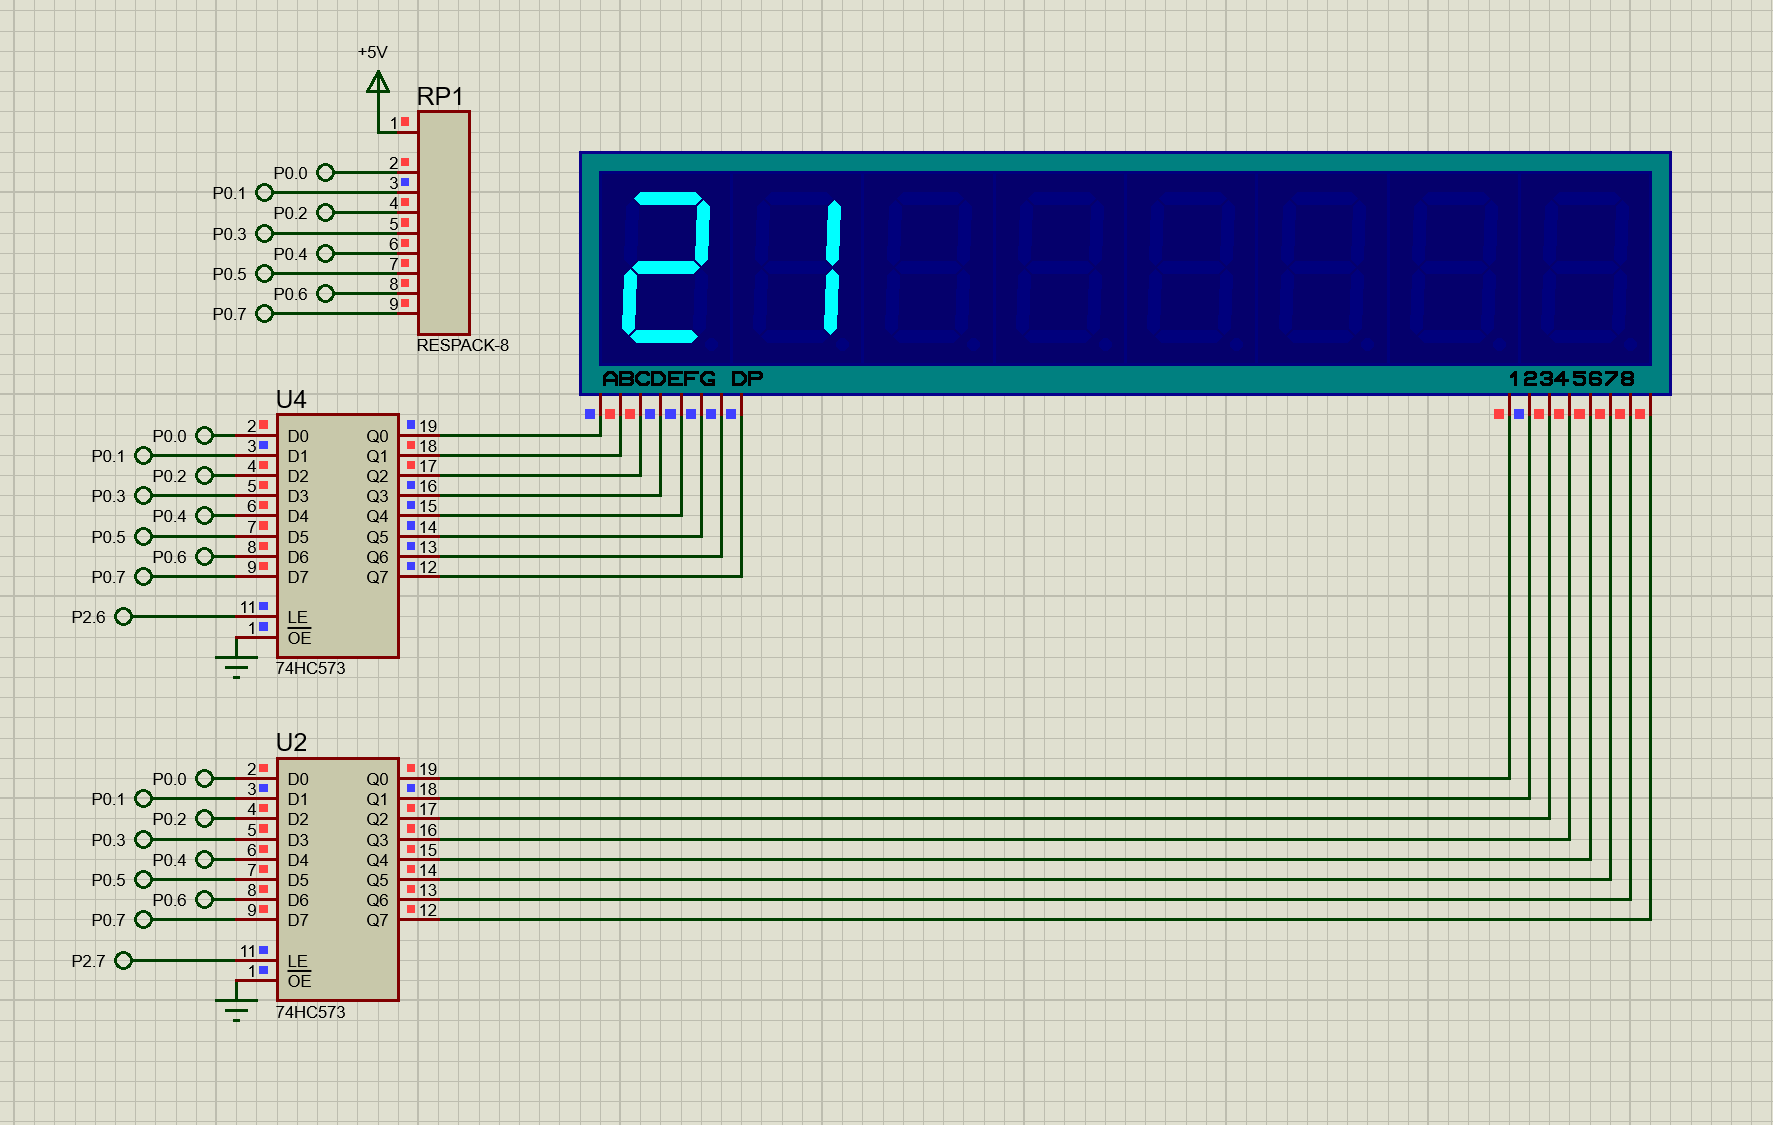
\includegraphics[width=0.84\textwidth]{images/lcd.png}
  \caption{两位温度显示与 74HC573 锁存电路}
\end{figure}

\subsection{端口分配}
\begin{table}[H]
  \centering
  \caption{AT89C51 与外设连接关系}
  \renewcommand{\arraystretch}{1.35}
  \begin{tabular}{p{0.24\textwidth}p{0.28\textwidth}p{0.38\textwidth}}
    \toprule
    单片机端口 & 外设连接 & 功能说明 \\
    \midrule
    P1.0--P1.7 & ADC0808 OUT8--OUT1 & 读取 8 位 A/D 转换数据，注意 OUT1 为高位 \\
    P2.1 & ADC0808 OE & 输出允许控制，高电平读取数据 \\
    P2.2 & ADC0808 START、ALE & 产生转换启动和地址锁存脉冲 \\
    P3.4 & ADC0808 EOC & 查询 A/D 转换结束状态 \\
    P0.0--P0.7 & 两片 74HC573 输入端 & 复用输出段码和位选码 \\
    P2.6 & 段码锁存 74HC573 的 LE & 锁存数码管段码 \\
    P2.7 & 位选锁存 74HC573 的 LE & 锁存数码管位选 \\
    \bottomrule
  \end{tabular}
\end{table}

\section{软件设计}

\subsection{程序设计思路}
程序采用“主循环刷新显示，定时中断周期采集”的结构。主循环不做复杂计算，只不断输出十位和个位的段码、位选码，保证数码管亮度稳定。定时器 0 工作在方式 1，按 50ms 进入一次中断，累计 20 次约为 1s。每满 1s 后，程序启动 ADC0808 转换、读取 P1 数据、近似换算温度，并拆分为十位和个位，供主循环显示。

\begin{figure}[H]
\centering
\resizebox{0.95\textwidth}{!}{%
\begin{tikzpicture}[
  node distance=8mm and 12mm,
  proc/.style={rectangle,rounded corners,draw=themecolor,fill=blue!3,minimum width=5.6cm,minimum height=8mm,align=center},
  term/.style={ellipse,draw=accentgreen,fill=green!8,minimum width=4.2cm,minimum height=8mm,align=center},
  line/.style={-Latex,thick,draw=themecolor}
]
  \node[term] (reset) {上电复位};
  \node[proc,below=of reset] (init) {初始化 P0/P1/P2、定时器 0 和中断};
  \node[proc,below=of init] (disp1) {输出十位段码和第一位位选};
  \node[proc,below=of disp1] (delay1) {短延时};
  \node[proc,below=of delay1] (disp2) {输出个位段码和第二位位选};
  \node[proc,below=of disp2] (delay2) {短延时};

  \draw[line] (reset) -- (init);
  \draw[line] (init) -- (disp1);
  \draw[line] (disp1) -- (delay1);
  \draw[line] (delay1) -- (disp2);
  \draw[line] (disp2) -- (delay2);
  \draw[line] (delay2.east) -- ++(1.0,0) |- (disp1.east);
\end{tikzpicture}}
\caption{主程序显示扫描流程图}
\end{figure}

\subsection{定时中断流程}
定时中断既负责 1s 采集周期，又避免在主循环中使用长时间等待。中断服务程序重新装载 TH0、TL0 后递减计数变量，若未满 1s 则直接返回；若计数到 0，则重新装载计数值并执行一次 ADC 采集和温度换算。

\begin{figure}[H]
\centering
\begin{tikzpicture}[
  node distance=8mm,
  proc/.style={rectangle,rounded corners,draw=themecolor,fill=blue!3,minimum width=7.4cm,minimum height=8mm,align=center},
  judge/.style={diamond,aspect=2.2,draw=accentyellow,fill=yellow!10,minimum width=4.4cm,minimum height=10mm,align=center},
  line/.style={-Latex,thick,draw=themecolor}
]
  \node[proc] (in) {进入 Timer0 中断，保护现场};
  \node[proc,below=of in] (reload) {重装 TH0/TL0，形成 50ms 定时};
  \node[judge,below=of reload] (cnt) {20 次是否到达};
  \node[proc,below=of cnt] (adc) {启动 ADC0808 并读取 P1 数据};
  \node[proc,below=of adc] (calc) {近似换算温度，拆分十位和个位};
  \node[proc,below=of calc] (out) {恢复现场并 RETI};

  \draw[line] (in) -- (reload);
  \draw[line] (reload) -- (cnt);
  \draw[line] (cnt) -- node[right,font=\small] {是} (adc);
  \draw[line] (adc) -- (calc);
  \draw[line] (calc) -- (out);
  \draw[line] (cnt.east) -- ++(1.0,0) |- node[right,font=\small,pos=0.25] {否} (out.east);
\end{tikzpicture}
\caption{1s 周期采集的定时中断流程图}
\end{figure}

\subsection{温度近似换算}
本实验的重点是掌握 ADC0808 的控制和数据显示，因此程序采用分段近似方式进行温度换算。对于 5k$\Omega$ NTC 与 10k$\Omega$ 上拉电阻组成的分压电路，25\,$^\circ$C 附近热敏电阻约为 5k$\Omega$，此时 ADC 数值约为：
\[
  D_{25} = \frac{5k}{10k + 5k} \times 255 \approx 85
\]
温度升高时 ADC 值变小，温度降低时 ADC 值变大。程序以 85 为分界点，分别使用线性近似，使显示值能够随采集电压变化而改变。该方法程序短、容易在 ASEM-51 下编译，适合实验验收；若进行实际测温，应进一步使用查表法或 Steinhart-Hart 方程进行标定。

\subsection{完整程序清单}
\lstset{style=a51style}
\lstinputlisting[caption={07\_temperature.A51 完整源程序}]{code/07_temperature.A51}

\section{仿真调试与结果分析}

\subsection{调试步骤}
\begin{enumerate}
  \item 检查 AT89C51 的电源、晶振、复位和 EA 引脚连接，确认单片机可以正常运行程序。
  \item 检查 ADC0808 的 VREF(+)、VREF(-)、CLOCK、START/ALE、EOC 和 OE 引脚，确认控制信号符合实验要求。
  \item 检查 ADC0808 的 OUT1--OUT8 与 P1 口的连接顺序。ADC0808 的 OUT1 为高位，OUT8 为低位，若位序接反，显示值会出现大幅跳变。
  \item 检查 ADD A、ADD B、ADD C 是否接地，确保固定选择 IN0 通道。
  \item 加载汇编生成的 HEX 文件，启动仿真，观察最左边两位数码管是否能够显示温度值。
  \item 改变热敏电阻模型或用电位器模拟热敏电阻阻值变化，观察显示温度是否随 ADC 输入变化而更新。
\end{enumerate}

\subsection{结果现象}
仿真运行后，最左边两位数码管能够稳定显示温度值。程序每 1s 进行一次 ADC 采样，因此改变模拟输入后，显示结果不会立即变化，而是在下一次采样周期到来后更新。显示部分采用动态扫描方式，主循环快速交替刷新十位和个位，因此肉眼观察为两位同时点亮。

\subsection{问题分析}
调试过程中需要特别注意两个问题。第一，ADC0808 数据位序必须与程序读取方式一致。8051 程序直接执行 \texttt{MOV A,P1}，默认 P1.7 为最高位、P1.0 为最低位；而 ADC0808 的 OUT1 为最高位、OUT8 为最低位，因此硬件连接应按高位对高位、低位对低位的方式处理。第二，用电位器模拟热敏电阻时，应保持分压模型清晰。若将固定电阻、电位器和热敏电阻全部串联，IN0 电压不再对应单一热敏电阻阻值，显示值会出现不易解释的跳变。

\begin{table}[H]
  \centering
  \caption{常见调试问题与处理方法}
  \renewcommand{\arraystretch}{1.35}
  \begin{tabular}{p{0.28\textwidth}p{0.34\textwidth}p{0.28\textwidth}}
    \toprule
    现象 & 可能原因 & 处理方法 \\
    \midrule
    数码管不亮 & 位选方向错误或锁存信号未连接 & 调整位选码，检查 P2.6/P2.7 \\
    显示值跳变很大 & ADC0808 输出位序接反 & 将 OUT1 接 P1.7，OUT8 接 P1.0 \\
    显示一直为 00 & IN0 电压超出程序换算范围或 OE 未打开 & 检查分压电阻和 P2.1 控制 \\
    调节电位器不线性 & 电位器与热敏电阻串联方式不当 & 用电位器单独模拟热敏电阻 \\
    采样无变化 & EOC 等待逻辑或 START 脉冲异常 & 检查 P2.2、P3.4 和 500kHz 时钟 \\
    \bottomrule
  \end{tabular}
\end{table}

\section{实验总结}

本实验完成了基于 AT89C51 和 ADC0808 的温度采集显示系统设计。硬件方面，系统包含单片机最小系统、NTC 热敏电阻分压电路、ADC0808 转换接口和两位数码管显示电路；软件方面，程序利用定时器中断实现 1s 采集周期，并在主循环中完成数码管动态扫描。通过本实验，进一步理解了 ADC0808 的启动、转换完成判断和数据读取过程，也认识到模拟量采集电路中分压电阻、位序连接和参考电压对结果准确性的影响。

实验中采用简化的分段线性换算实现温度显示，能够满足课堂验收中“采集、转换、显示”的功能要求。若将该系统用于更高精度的实际温度测量，还应根据热敏电阻的具体参数进行标定，并使用查表或非线性公式提高温度换算精度。


\end{document}
